\documentclass[a4paper,11pt,oneside]{book}

% packages 
\usepackage{arsclassica}    % fancy layout
\usepackage[english]{babel}\addto{\captionsenglish}{\renewcommand{\bibname}{References}}
\usepackage{caption}         % figure captions
\usepackage[square,numbers,super,sort&compress]{natbib}  % bibliography style
\usepackage[cc]{titlepic}    % enable logo on title page
\usepackage{graphicx}       % logo related

\usepackage{standalone}
\standalonetrue

% Margins for pretty version ::
%\usepackage[pass]{geometry}
% Margins for university regulations ::
\usepackage[top=2cm, bottom=4cm, left=4cm, right=2.5cm]{geometry}
\usepackage{setspace}
\onehalfspacing

% don't hang captions
\captionsetup{format=plain}

% bibliography
\bibliographystyle{../thesis}

% title setup
\title{ \vspace{3in} Unravelling higher order genome organisation {\small [working
    title]} \\ \vspace{2em} {\large {\bf Introduction}} }
\author{Benjamin L. Moore}
\titlepic{\vspace{2.2in} 
\includegraphics[width=\textwidth]{/Users/benmoore/hvl/1yrReport/figs/igmm.png}}

\begin{document}

%\maketitle

\chapter{Introduction}
\section{Genome organisation}\label{intro:genomeorg}
%
It's oft-stated that the DNA within each human cell would extend for two metres fully extended. Instead that same length of DNA packs into a cell nucleus with a diameter in the order of micrometers ($\mu$m). This is achieved through a complex organisation hierarchy, ranging from how chromosomes are arranged in the nucleus in territories, to chromatin interactions with the nucleolus or nuclear periphery, down to how DNA is wrapped around nucleosomes (for recent reviews, see \citenum{Pombo2015, Fraser2015}). While the biophysics of the latter level of organisation may be well understood, more broadly there is still much to learn about the guiding principles and functional importance of higher order chromatin organisation.

This introductory section will describe the current state-of-the-art in chromosome conformation capture experimental methods, as well as criticisms and considerations when interpreting these data, and discuss what is currently understood or theorised about the structure and function of higher order genome organisation. We compare competing models which attempt to recapitulate mechanisms of chromatin folding, and also explore some of the best understood organisational strata in mammalian higher order genome organisation.

%
%Briefly, DNA exists mostly as a left-handed double-helix of hydrogen bonded purines and pyrimidines. These in turn are wrapped around histone octamers, proteins with tuneable DNA packing properties. These wrapped histones can be visualised as "beads on a string" in transcriptionally active regions, and possibly as a more-compact 30 nanometre fibre, though this is disputed.\cite{Naumova2013} %citations therein

\subsection{C-methods and Hi-C}

Classical studies of chromosome conformation relied on microscopy techniques to visualise nuclear architecture, most commonly fluorescence \emph{in situ} hybridisation (FISH). These techniques led to the discovery of ``chromosome territories", regions of the nucleus wherein distinct chromosomes were thought to occupy, and more broadly identified the non-random arrangement of loci in three-dimensional space.\cite{DeWit2012, VanSteensel2010} Finer details of chromatin organisation, such as the proposed 30 nm fibre, were also introduced through microscopy-based techniques. Techniques such as FISH are powerful for precise inspection of single genes, but are low-throughput and offer limited resolution.\cite{DeWit2012}

With the advent DNA sequencing technology, new experimental methods emerged. Chromosome conformation capture (3C), introduced by Dekker \emph{et al.}\cite{Dekker2002} was the first sequencing-based method of assaying nuclear architecture. The 3C method uses formaldehyde to cross-link nuclear proteins in place, trapping genomic regions that were physically co-located through bound proteins, then a frequent-cutter restriction enzyme shears the sample into DNA fragments. Next, under dilute conditions, these fragments are ligated together. The dilute conditions favour ligations between fixed fragments, with the aim of generating hybrid fragments from genomic regions which were close together in the original preparation. Cross-linking can then be reversed and, in the case of the original 3C method, measured by quantitative PCR using pre-designed primers for your fragments of interest. The end result is a relative measure of interaction frequency between any two regions of interest, in theory directly proportional to their distance in three-dimensional space.

Rapid advancements in sequencing technology allowed the original 3C method to be further developed, first through microarrays, then using high-throughput sequencing. Two protocols were proposed for a 3C-inspired one-to-many assay\cite{Zhao2006, Simonis2006} (both named 4C), whereby interactions were measured for a specific ``viewpoint" fragment against all other restriction fragments genome-wide. The same year a many-to-many assay (5C) allowed measurements for all restriction fragments within a specified region.\cite{Dostie2006} 

The final stage in the evolution of the 3C method was an all-versus-all assay, capable of assaying pairwise interaction frequencies between all restriction fragments of a genome. Such an assay was published by Lieberman Aiden \emph{et al.}\cite{Lieberman2009} and named Hi-C (Fig. \ref{fig:hicmethod}). The Hi-C method added biotin tagging to pull-down only ligated fragments for sequencing. At the time of the assay's publication, resolution of Hi-C data for analysis was limited by sequencing depth---of particular concern given the enormous pairwise interaction space between all restriction fragments produced by a 6-cutter enzyme---but the falling costs of sequencing and proven utility of the assay meant subsequent Hi-C papers incrementally upped their sequencing depth, culminating at the time of writing to the point where analyses are starting to be performed at the level of individual restriction fragments, genome-wide.\cite{Dixon2012,  Selvaraj2013a, Jin2013, Rao2014}

\begin{figure}
\begin{center}
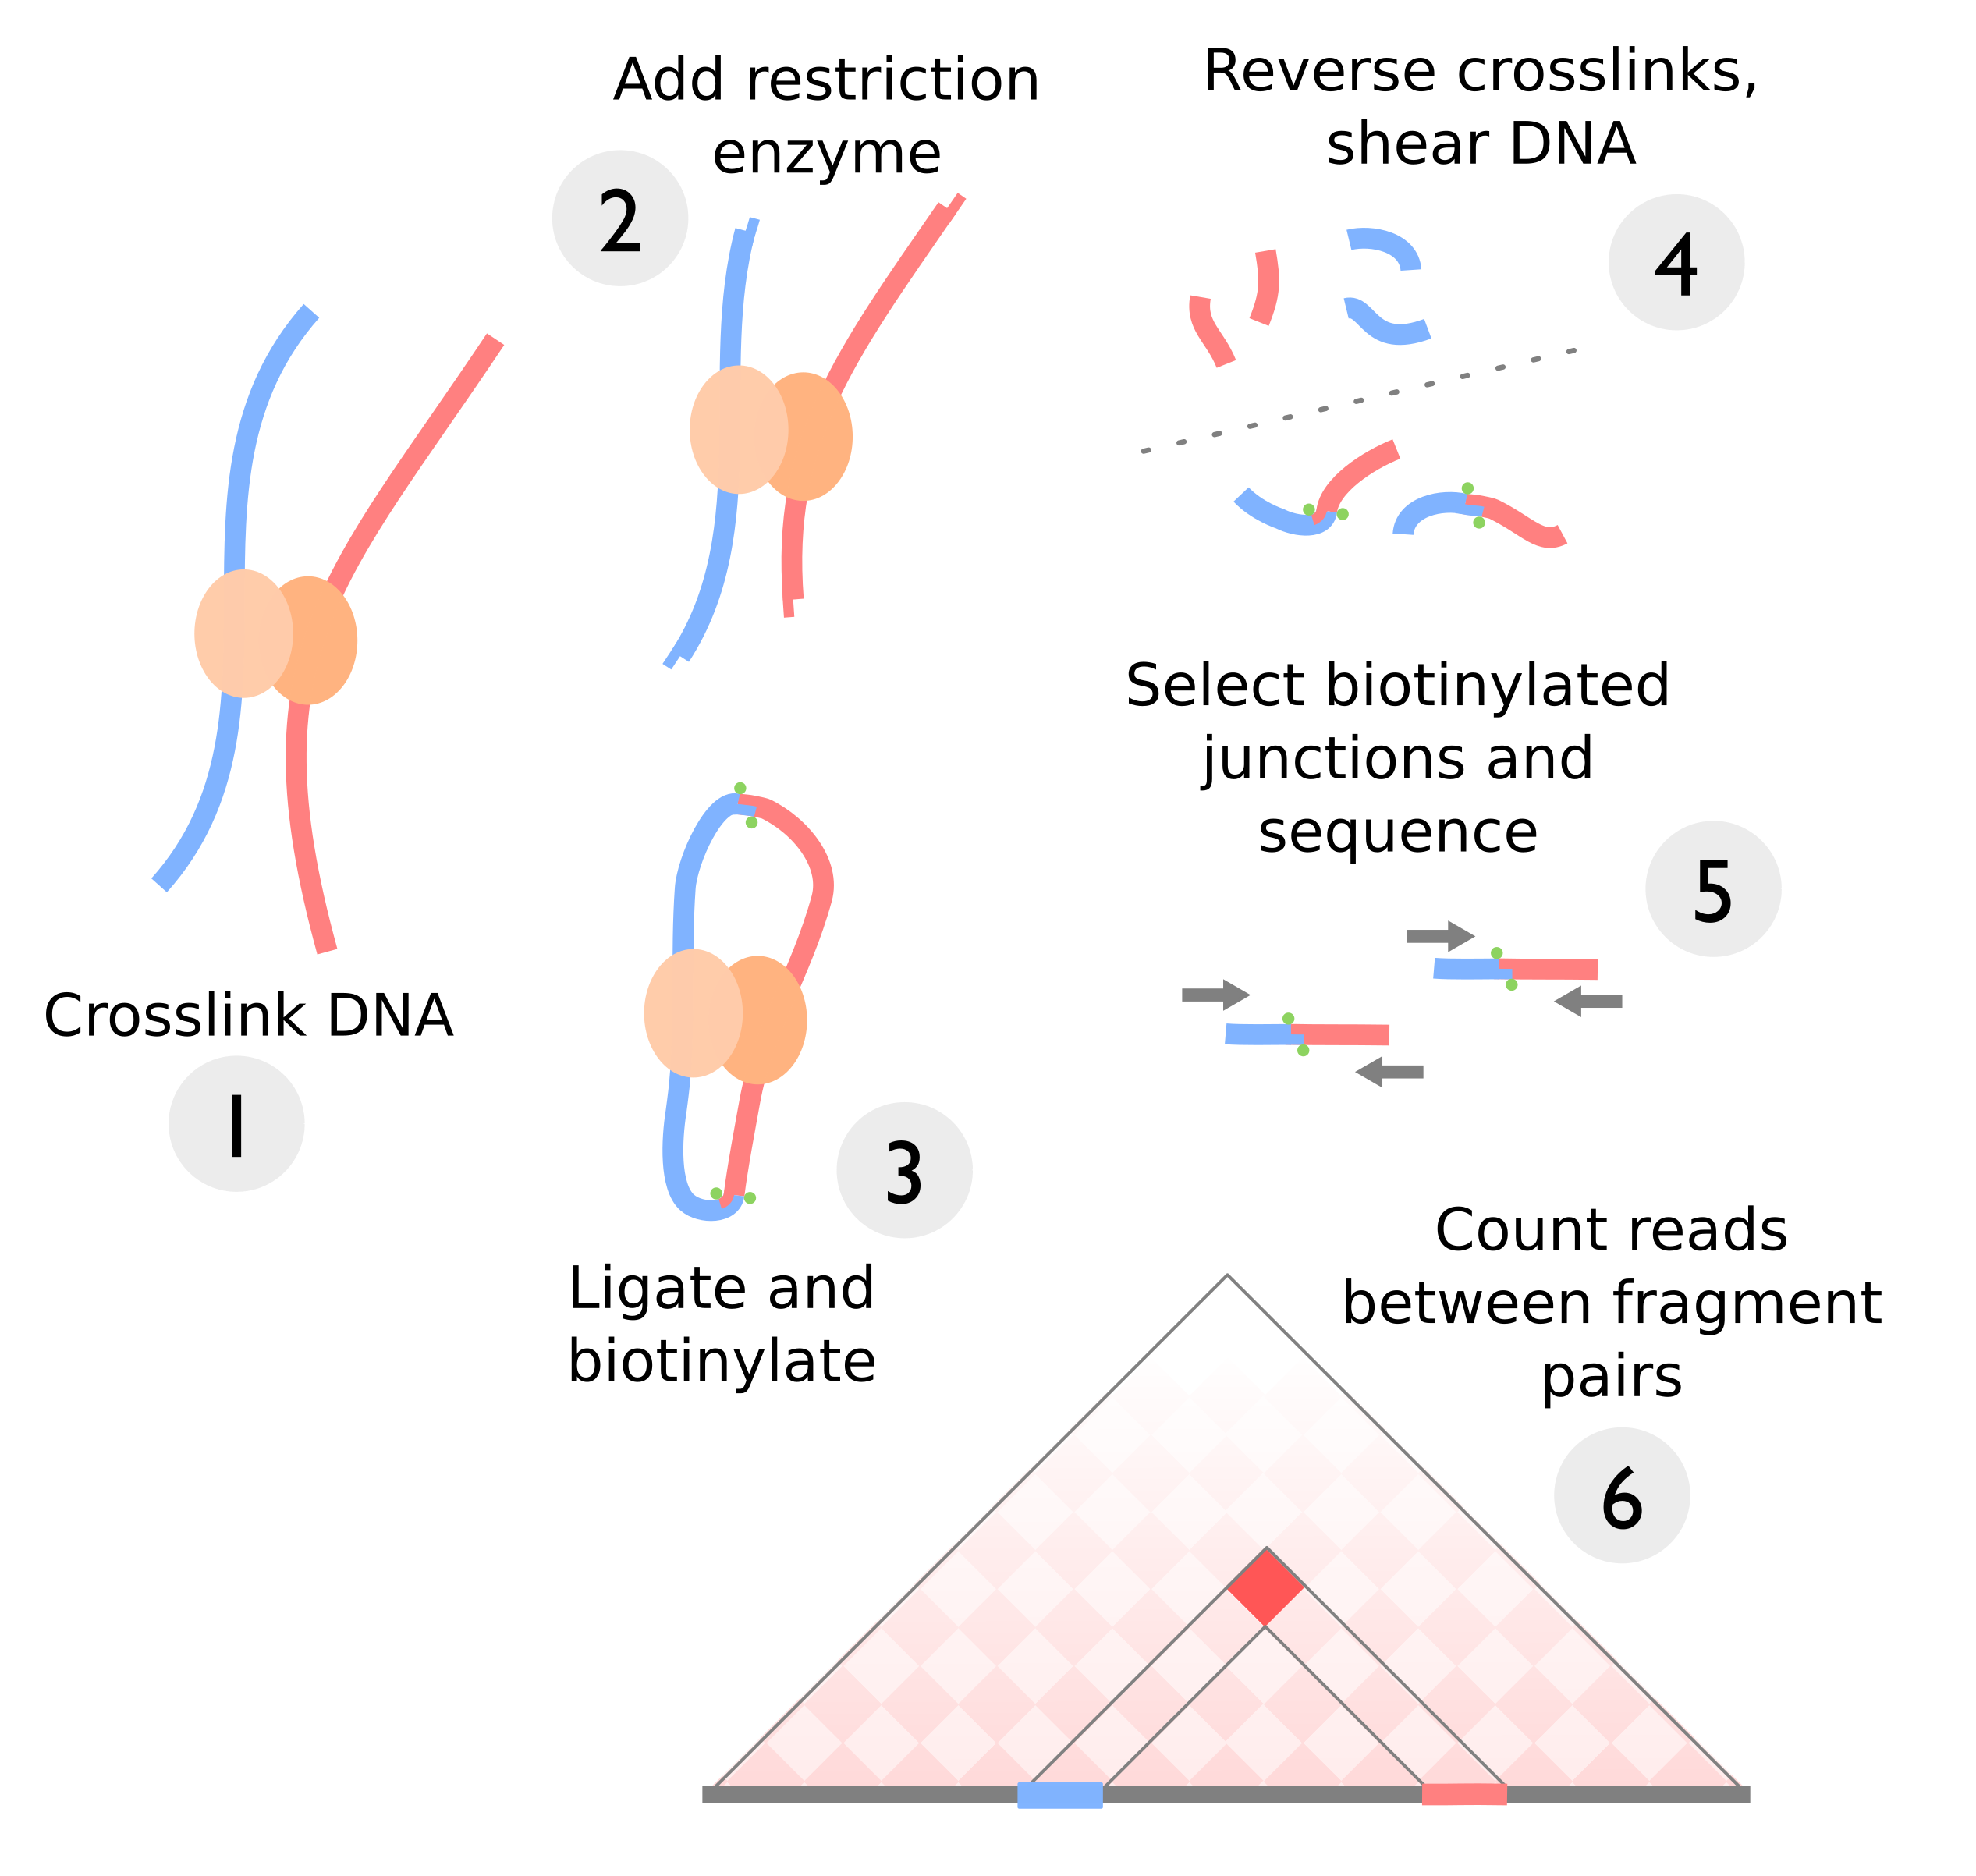
\includegraphics[width=4in]{figs/hic.png}
\captionsetup{width=\textwidth}
\caption[Steps in the Hi-C assay.]{ {\bf Steps in the Hi-C assay. } 
  Schematic of the Hi-C experimental procedure as described in \citet{Lieberman2009}
}\label{fig:hicmethod}
\end{center}
\end{figure} 

\subsection{Hi-C variants}\label{sec:hicvar}

The interaction maps produced by Hi-C were found to contain several inherent biases. Restriction fragment properties, such as their length, GC content and mappability, were confounding interaction frequency estimates and therefore needed to be normalised-away before subsequent analysis.\cite{Yaffe2011, Hu2013} A range of statistical techniques were developed to correct for these latent variables,\cite{Imakaev2012, Dekker2013, Hu2012, Li2014} while experimentalists instead looked to improve on the experimental procedure itself.

Tethered chromosome capture (TCC)\cite{Kalhor2012} was the first attempt to increase the signal to noise ratio of Hi-C contacts. In this method, ligations take place on a fixed surface, with the aim of preventing spurious ligations between fragments in solution which were not cross-linked. Kalhor \emph{et al.}\cite{Kalhor2012} reported a large decrease in observed interchromosomal contacts in their tethered library, suggesting many of those originally observed were caused by spurious ligation of non-crosslinked fragments.

\emph{In situ} Hi-C is another, more recent refinement of the Hi-C method from some of those who developed the original Hi-C method.\cite{Rao2014} In contrast to TCC, fixation and ligation now happen in place within intact cell nuclei. The observed improvements with this \emph{in situ} procedure, however, are similar: interactions are assayed with greatly reduced noise and again many fewer \emph{trans} contacts are reported.\cite{Nagano2015}

Hi-C and the variants introduced thus far are population-level assays, reporting summed interaction counts over a cell population. As well as building population-averaged models of genome structure, it is also of interest to probe cell-to-cell variability through single-cell approaches. For instance, it's been estimated that long-range contacts identified with C-methods may occur in as few as $10\%$ of cells at any one time.\cite{VanSteensel2010} 

In the first single-cell Hi-C study, Nagano \emph{et al.}\cite{Nagano2013} aimed to explore this cell-to-cell variability by performing the Hi-C assay on single, hand-selected nuclei. An obvious limitation of this Hi-C variant is that a single restriction fragment can ligate to at most one other fragment per experiment, meaning even if $100\%$ yield were to be achieved, any $n \times n$ restriction fragment interaction matrix could have at most $\frac{n}{2}$ nonzero entries; in practice, the realised yield of this first single cell Hi-C experiment was just $2.5\%$.\cite{Nagano2013} Nevertheless, single-cell Hi-C was able to reproduce findings from population-based (or ``ensemble") Hi-C, such as preferential interactions between active domains, and also was able to dissect \emph{trans} interactions, suggesting high cell-to-cell variability leads to their relatively uniform appearance in normal Hi-C interaction maps.\cite{Nagano2013} When combined with the observations of TCC and \emph{in situ} Hi-C, which gave evidence that interchromosomal contacts were disproportionately the result of spurious ligation,\cite{Kalhor2012} the functional significance of these \emph{trans} interactions seems at best unclear in the general case.

Capture-C is an altogether different Hi-C variant which attempts to address the resolution problems associated with the standard assay by enriching for functional interactions using \emph{a priori} selection for loci of interest.\cite{Hughes2014} Indeed, a suggestion in the original Hi-C paper was that resolution could be improved by either increased sequencing or using hybrid capture.\cite{Lieberman2009} Since the release of Capture-C, more Hi-C variants with a target enrichment step have been developed, including Capture Hi-C (CHi-C)\cite{Dryden2014} and HiCap.\cite{Sahlen2015} These methods have been applied to genome-wide target sets (e.g. CHi-C assayed $22,000$ human promoters\cite{Mifsud2015}) and so it could be said that they are to Hi-C as exome-capture is to whole-genome sequencing, in the contexts of chromosome conformation capture and variant discovery respectively. 

%Use of a cell population also averages away cell-cycle effects, with the vast majority of results coming from cells during interphase (around $97\%$\cite{Naumova2013}). Naumova \emph{et al.}\cite{Naumova2013} looked to assay chromosome conformation specifically over different cell cycle stages, to better understand chromosome compaction during mitosis.


% DNase Hi-C

\subsection{Chromosome compartments}\label{sec:compartments}

In the paper describing the Hi-C technique, \citet{Lieberman2009} described low-resolution structures they name  ``A'' and ``B'' nuclear compartments. These are genomic regions with a median size of around 5 megabases which showed properties typical
of euchromatin and heterochromatin, respectively. A compartments were observed through 3D-FISH to be centrally-positioned in the nucleus and  ChIP-seq data showed several hallmarks of transcriptional activity. B compartments, conversely, were heterochromatic and often lamina-associated regions, with little transcription and repressive histone modifications such as H3k9me3.\cite{Lieberman2009, DeWit2012} 
%As expected from positioning data, the co-location of compartment types is also visible in their contact maps. 

\begin{figure}
\begin{center}
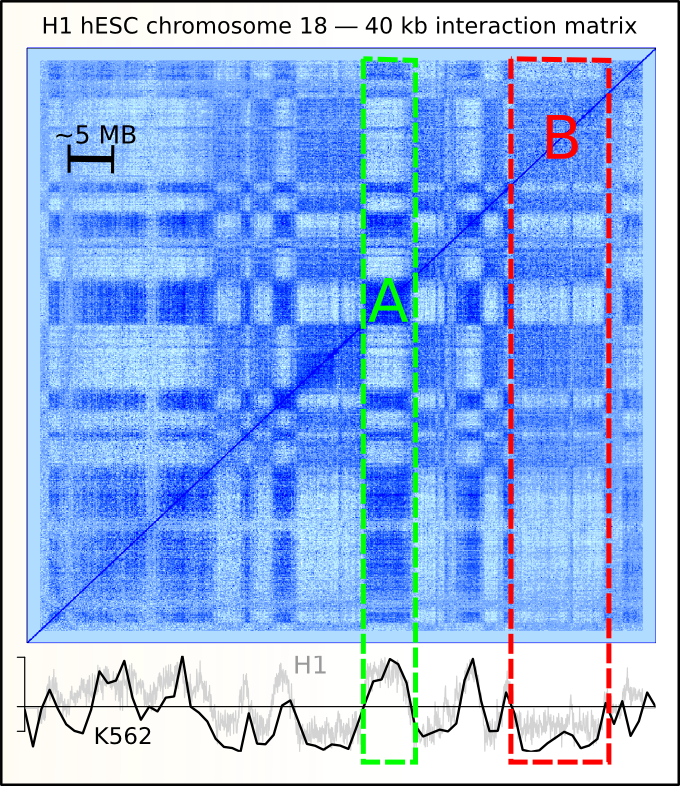
\includegraphics[width=.75\textwidth]{figs/eigcalc.png}
\captionsetup{width=\textwidth}
\caption[Derivation of an A/B compartment profile from Hi-C data.]{ {\bf Derivation of A/B an compartment profile from Hi-C data.} 
Intrachromosomal observed interaction frequencies (O) are averaged along super-diagonals to give a distance-normalised expected matrix (E). The Pearson correlation of the O/E matrix then can undergo eigenvector expansion; in most cases eigenvector $\mathbf{v}$ with the largest eigenvalue, $\lambda$, then reflects A/B compartmentalisation.\cite{Lieberman2009} Matrices are coloured from blue (lowest values), through yellow, to highest values in red.
}\label{fig:eigcalc}
\end{center}
\end{figure} 

These A and B  compartments were identified through a continuous principle component eigenvector profile, derived from a normalised Hi-C contact matrices\cite{Lieberman2009} (Fig. \ref{fig:eigcalc}). This approach can be intuitively understood as formulated by \citet{Lajoie2014}:
\begin{enumerate}
\item A tartan pattern on normalised Hi-C matrices indicates two preferentially-contacting and exclusive compartments (Fig. \ref{fig:eigcalc}).
\item Assume a function ($c$) that maps a given genomic bin to its compartment, using a positive number for compartment A and a negative for compartment B.
\item The interaction frequency between bins $i$ and $j$ is thus $c(i)\cdot c(j)$. (Note that this rule alone is sufficient to generate a tartan pattern: if $i$ and $j$ are in the same compartment, the product will be positive, and for compartments of opposing type, negative.\cite{Lajoie2014})
\item Our symmetric Hi-C matrix thus contains $c(i)c(j)$ and in this formulation, principle components analysis is finding the basis that minimises the mean-squared error between $c(i)c(j)$ and $c(i)$.
\end{enumerate}
Importantly, this measure holds more information than a simple two-state classification, rather the continuous values can be interpreted as relative levels of compartment identity, hence degrees of compaction or activity.\cite{Dekker2013, Imakaev2012}

\subsection{Topologically associating domains}\label{intro:tads}

The falling cost of high-throughput sequencing has enabled increasingly deep sequencing of Hi-C experiments. Sequencing depth is the main resolution-limiting resource for this assay; in order to increase the analysis resolution while maintaining the same level of coverage requires an exponential increase in the total amount of sequencing.\cite{Lieberman2009, Tanay2013} Nevertheless such deep sequencing has 

In experiments totalling around two billion total sequencing reads, \citet{Dixon2012} produced Hi-C contact maps in human and mouse cell lines at 40 kb resolution. At the same time, \citet{Nora2012} published an even higher-resolution 5C dataset covering a $4.5$ Mb region of the mouse X chromosome. In both of these studies, the authors uncover what are now known as "topologically associating domains" (or TADs), observable as off-diagonal blocks in a contact map which exhibit higher-than-expected self-interaction frequency. With a mean size of around 1 Mb, TADs were recognised as a novel layer of higher order chromatin organisation at a level below the larger A/B compartments (Section \ref{sec:compartments}). TADs have since been reported in a variety of metazoan organisms including dog,\cite{VietriRudan2015} \emph{Drosophila}\cite{Sexton2012, Hou2012} and \emph{C.~elegans}\cite{Crane2015} yet comparable structures are not found in higher plants such as \emph{Arabidopsis}\cite{Feng2014, Wang2015} or in yeast.\cite{Duan2010, Gong2015}

\citet{Dixon2012} defined a TAD calling algorithm based on the directional bias of a genomic region's contacts, and used a hidden Markov model to infer blocks of strongly up- or downstream-biased, reasoning that domain boundaries are present when a strongly upstream biased region is adjacent to a region of opposite bias (Fig. \ref{fig:dicalc}). These boundaries themselves were investigated and found to show suggestive functional enrichments for DNA binding proteins including CTCF, long thought to act as an insulator of chromatin state (Section \ref{intro:loops}). Deletion of a  CTCF site has been found to disrupt the corresponding TAD border, while removal of some other enriched factors had little effect.\cite{Nora2012, Zuin2013, Narendra2015}
\citet{Dixon2012} also performed some comparative analysis, reporting large and significant overlap of domain boundary positions both within species and between human and mouse.

\begin{figure}
\begin{center}
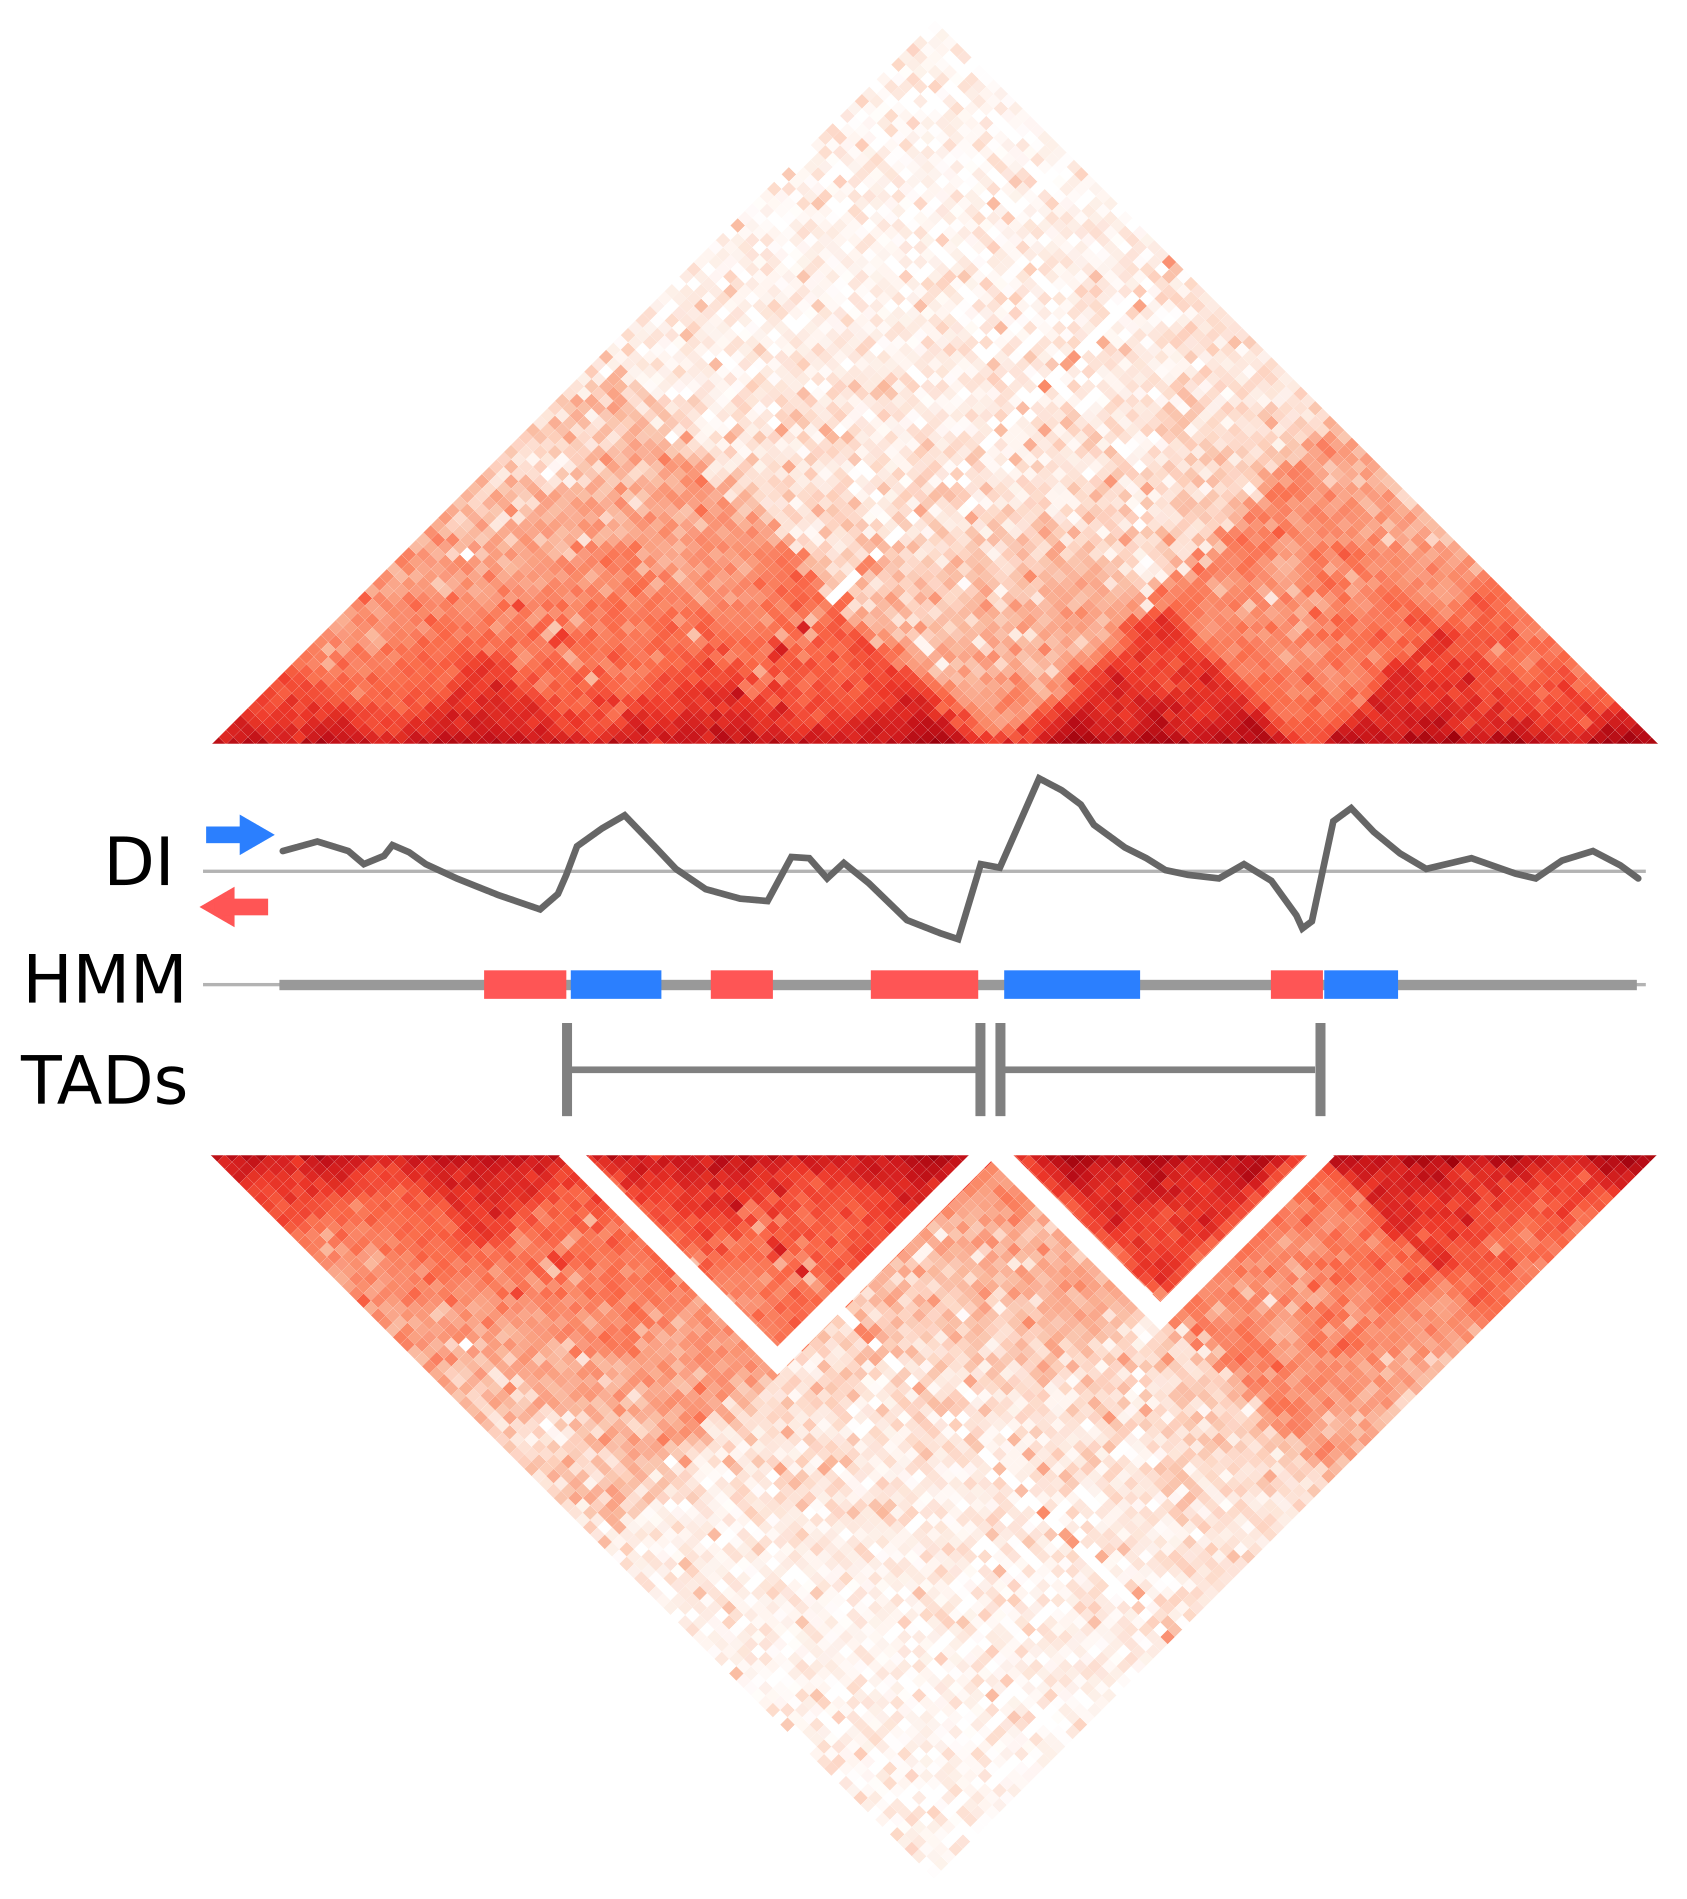
\includegraphics[width=2.5in]{figs/di_example.png}
\captionsetup{width=\textwidth}
\caption[Dixon \emph{et al.} pipeline for calling topologically associating domains.]{ {\bf Dixon \emph{et al.} pipeline for calling topologically associating domains.} First a directionality index (DI) is calculated for each bin based on the ratio of upstream:downstream contacts. Secondly a hidden Markov model (HMM) is used to infer the most likely state sequence that emitted the DI variable. Finally a simple rule is applied whereby a run of high-confidence upstream-biased state calls marks the end of a domain. New domains begin with any subsequent downstream-biased state. Gaps between TAD calls can be observed and these are labelled border regions up to a size threshold of 400 kb, whereafter those regions are unclassified.\cite{Dixon2012} Additional details are given in Methods \ref{meth:tadcalling}.
}\label{fig:dicalc}
\end{center}
\end{figure} 

% Function of TADs, regulons, hormone treatment, differentiation etc.
% Sexton2015 review
Since then, several studies have investigated the functional implications of TADs. A simple biological explanation is that TADs delimit functional contacts, such as those between enhancers and promoters, and so could inhibit spurious contacts with other nearby genetic elements.\cite{Fraser2015, Sexton2015} Moreover, hormonal treatment of human breast cancer cells reported coordinated expression responses within TADs, suggesting they also function as domains of transcriptional co-regulation called "regulons".\cite{LeDily2014} However the size of TADs means they often span multiple genes, commonly with unrelated functions, so it seems unlikely they can function as regulons in the general case.\cite{Pombo2015} At the time of writing, the functional significance of TADs is the subject of ongoing debate within the chromatin biology field.

\subsection{Other proposed structures}

Since the discovery of TADs, multiple publications have proposed either complementary or altogether different classes of chromatin domains. For example, \citet{Filippova2014} developed a tuneable algorithm which identifies "alternative topological domains". The authors use dynamic programming to search for an optimal set of non-overlapping boundary pairs that maximise intra-domain contacts. The algorithm includes a length scaling factor ($\gamma$) which is used to penalise domain size; by varying $\gamma$ the authors define a subset of "multiscale domains" of heightened persistence across resolutions.\cite{Filippova2014} These multiscale domains were found to be smaller, on average, than those previously reported by \citet{Dixon2012}, even when applied to the same Hi-C experimental data (with a mean size of 200 kb as opposed to $\approx 1$ Mb). However the domains of \citet{Filippova2014} show increased intra-domain contacts and stronger boundary enrichments relative to previously-described TADs, indicating this algorithm may generate a more accurate representation of topological domains in mammalian genome organisation. Intriguingly, this study also reports quantitative evidence for hierarchical genome organisation, finding that those domains called at large $\gamma$ will then combine into larger meta-domains as the $\gamma$ penalty decreases.\cite{Filippova2014}

A study of \emph{Drosophila} embryonic chromosomes found a similarly hierarchical organisation of physical domains, and also was able to relate these to ``epigenomic domains" which exhibited specific sets of enrichment signatures representing active, null, polycomb-associated and telomeric regions.\cite{Sexton2012} This study provided evidence for the first time that contact domains are linked with average epigenomic enrichments.

Recent high-resolution studies have been able to resolve ever-smaller levels of sub-structure. Rao \emph{et al.}\cite{Rao2014} refined the concept of chromosome compartments to "sub-compartments", dividing simple A/B divisions into a total of 5 subtypes. The authors were also able to identify "contact domains" of median size 185 kb, many of which were associated with identifiable individual looping events (Section \ref{intro:loops}).\cite{Rao2014} This domain size is close to those of \citet{Filippova2014} (described above) and the authors here suggest that previously-observed large TADs may be the result of insufficient sequencing; that is, not all boundaries could be detected using 40 kb binned contact maps thus multiple contact domains were unintentionally combined into large domains. Additionally, these sub-compartment types exhibit average epigenomic enrichments along the lines of those reported in \emph{Drosophila} by \citet{Sexton2012} and so potentially provide an overarching concept that connects TADs, alternative domains and epigenomic domains.

\section{Models of chromatin folding}

Theoretical mechanistic models of chromatin folding such as the
``strings and binders switch'' model\cite{Barbieri2012} and the ``fractal
globule'' model\cite{Lieberman2009, Mirny2011, Grosberg1988a} have both produced simulated data
that reflects empirical C-method observations and thus potentially describe the polymer
dynamics of chromatin folding.

\begin{figure}
\begin{center}
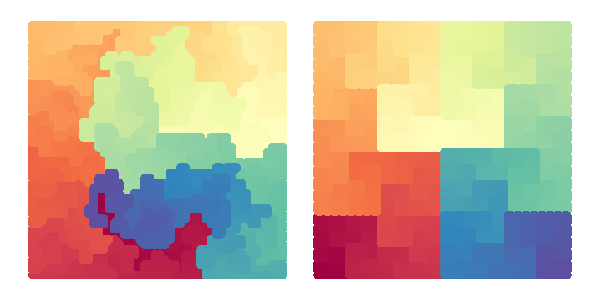
\includegraphics[width=5.5in]{figs/fractals.pdf}
\captionsetup{width=\textwidth}
\caption[ Comparison of theoretical models of chromatin folding. ]{ {\bf Comparison of theoretical models of chromatin folding. } 
 Two theoretical models of chromatin folding are shown simulated along a 2D polymer, coloured from start to finish as blue--green--red. An equilibrium globule is represented by a Hamiltonian path through a grid network (\emph{left}) and is compared to a fractal globule model, here represented by a Hilbert curve (\emph{right}).
}\label{fig:fractals}
\end{center}
\end{figure} 

\subsection{Fractal globule}
\citet{Lieberman2009} tested a number of theoretical models of genome folding to see which best explained the observed power-law scaling between distance and interaction frequency ($\textrm{IF} =  \frac{1}{dist^{-\alpha}}$ where $\alpha \approx 1.08$).  The authors sought to distinguish between two models of genome organisation: the previously-described "fractal globule"\cite{Grosberg1993, Grosberg1988a} and a less-structured "equilibrium globule" (Fig. \ref{fig:fractals}). The study found that a theoretical fractal globule, embodying scale-independent and self-similar aggregate folding, better fit the observed data than an equilibrium globule null model where simulated polymer folding was allowed to proceed unchecked.

% cartoon of fractal globule ?
% Dekker2013 has details on these, e.g. vs. equilibrium

The fractal globule model was noted for its appealing functional properties. Under this model, for example, the polymer folds are knot-free hence could facilitate local dynamics of repression and activation without wider disruption.\cite{Mirny2011} Despite this appeal, the authors were careful to state that while their simulations show good agreement with observed data, this does not preclude other organisational models from having similar or greater explanatory power.\cite{Lieberman2009}

\subsection{Strings and binders switch}\label{intro:sbs}

Subsequent modelling techniques integrated known biological phenomena as well as polymer models. This idea formed the basis of Barbieri \emph{et al.}'s\cite{Barbieri2012} ``strings and binders switch" (SBS) model, where the authors simulated polymer folding in the presence of DNA binding factors, such as the known genome architectural protein CTCF (Section \ref{intro:loops}). The SBS model was developed in an attempt to consolidate global Hi-C measures of contact scaling with those values from C-based experiments on smaller regions and FISH studies, which report a range of scaling parameters. The authors also explore the different observed values of $\alpha$ between cell lines and even chromosomes, and find that their mechanistic model can explain each case using variable concentrations of binders which cause phase-switching between accessible and compacted chromatin, with a fractal globule organisation existing at the phase transition boundary.\cite{Barbieri2012}

This SBS model achieves broad explanatory power for a range of observed power law coefficients ($\alpha$), and does so from simple underpinnings, but critics point out that simulations were performed on a polymer composed of just 512 monomers so may not be broadly applicable.\cite{Dekker2013}

\subsection{Looping and CTCF}\label{intro:loops}

\begin{figure}
\begin{center}
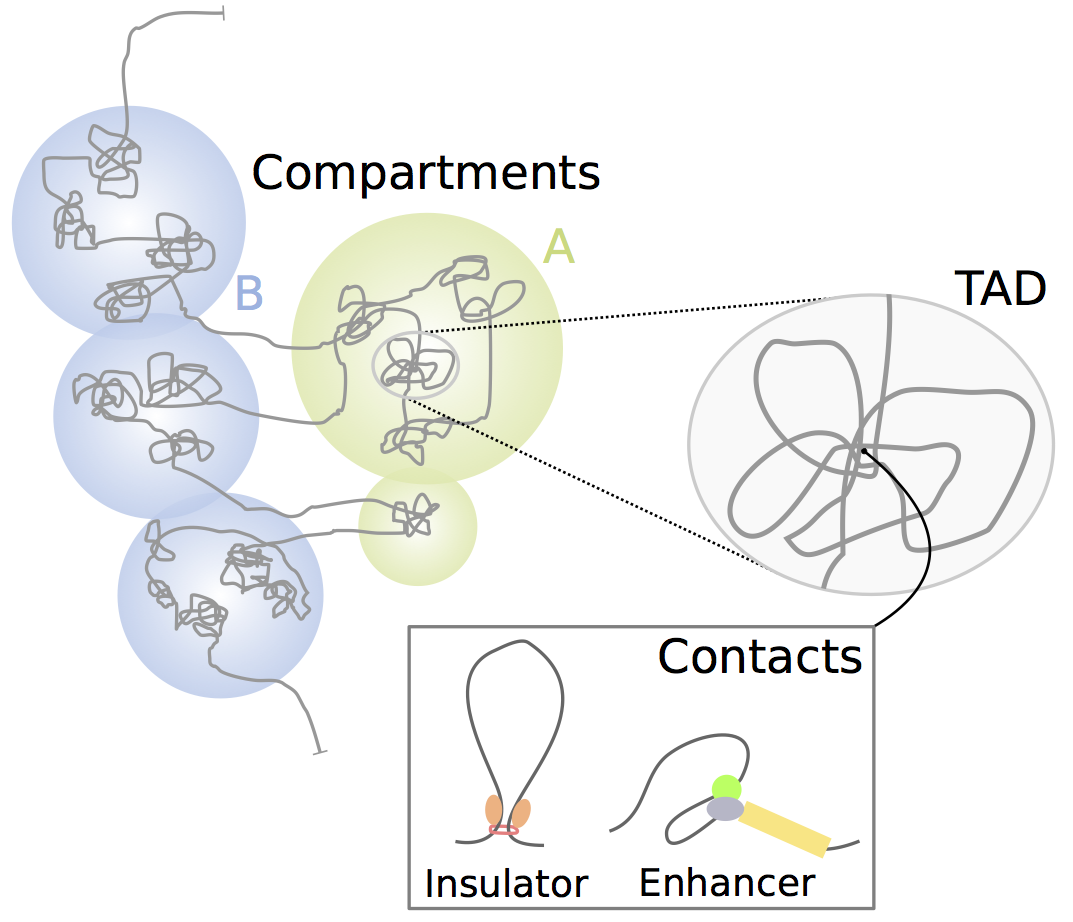
\includegraphics[width=4in]{figs/genome_org.png}
\captionsetup{width=\textwidth}
\caption[Levels of higher order chromatin organisation.]{ {\bf Levels of higher order chromatin organisation. } 
  Cartoon showing how functional contacts, such as loops between bound CTCF insulators (Section \ref{intro:loops}), occur within TADs (Section \ref{intro:tads}) which in turn are found within A or B compartments (Section \ref{sec:compartments}).
}\label{fig:genomeorg}
\end{center}
\end{figure} 

Examples have long been known of specific enhancer elements that are brought into close proximity with the promoter(s) they are regulating; under this model, these contacts form a "loop" structure between two potentially distal loci\cite{Kadauke2009a, Sexton2009} (Fig. \ref{fig:genomeorg}). A model region, the $\beta$-globin locus and its locus control region (LCR) located 40-80 kb away,\cite{Dekker2013} has been studied since the early 1980s,\cite{Banerji1981, Engel2000, Blackwood1998, Tolhuis2002} and is an interesting example of a well-characterised looping event. Current knowledge suggests the $\beta$-globin locus forms loops with the multiple distal \emph{cis}-enhancer elements that make up the LCR, forming an active chromatin hub (ACH).\cite{VandeCorput2012a} Within such a hub, regulatory signals could be efficiently integrated to dictate the overall activity of the target locus.\cite{DeWit2012, Pombo2015} It is now thought that the majority of active promoters are engaged with multiple, often cell type specific, regulatory looping events.\cite{Sanyal2012, Jin2013}

A notable component of many long-range looping events is the CCCTC-binding transcription factor (CTCF),\cite{Ong2014, Phillips2009, Handoko2011} already mentioned as a component of TAD boundaries (Section \ref{intro:tads}) and as a proposed looping factor in the SBS model (Section \ref{intro:sbs}). CTCF is strongly conserved in higher eukaryotes,\cite{Filippova1996a} ubiquitously expressed and embryonic lethal, but it is not tied to a single biological function --- instead CTCF has been described as a "multivalent factor",\cite{Phillips2009} capable of regulating transcription, imprinting, dosage-compensation and acting as an insulator. 

In the context of genome organisation, CTCF is of interest for its role of anchoring interactions between loci, forming loops. Experimental evidence has shown that interactions between CTCF sites stabilises the aforementioned loops linking the $\beta$-globin locus with its distal LCR.\cite{Splinter2006} This looping role, potentially undertaken in combination with other architectural proteins such as Mediator and cohesion,\cite{Phillips-Cremins2013, Sexton2009} can explain its previously-identified insulator behaviour: CTCF can block the spread of heterochromatin and contacts between enhancers and promoter through topological constraints by forming loops.\cite{Phillips2009} It must be said, however, that the functional significance of CTCF-mediated loops, and indeed the role of CTCF in even well-studied systems, remains only partially understood.\cite{Gomez-Diaz2014}

% bring back around to Rao2014 via CTCF
A recent Hi-C paper, that of Rao \emph{et al.},\cite{Rao2014} again brought CTCF and looping to the fore of chromatin conformation research. This study identified around $10,000$ individual looping events in the human genome, almost all linking loci over distances of less than 2 Mb, and around $30\%$ connecting predicted enhancer and promoter chromatin states. \citet{Rao2014} also report a 6-fold overall increase in expression when comparing those promoters participating in a looping event with those not. Furthermore, $86\%$ of these loops involved CTCF bound regions, with roughly the same overlapping proportion involving cohesion subunits RAD21 and SMC3. The authors thus propose that a CTCF-binding motif can act as an "anchor", which can then be bound by a transitive complex of other architectural proteins.\cite{Rao2014} A majority of these loops ($65\%$) also demarcated a topological domain, and at much higher resolution than previously observed (Section \ref{intro:tads}). Another striking finding of this research was that CTCF loops almost always occur in between bound motifs with a convergent orientation,\cite{Rao2014} though questions remain over why this should be the case, especially when considering the interactions of a flexible polymer in 3-D solution.\cite{Nichols2015}

% recently partially addressed with http://www.sciencedirect.com/science/article/pii/S0092867415009691 + Guo et al. (2015) in Cell

While the evidence linking CTCF and genome architecture is substantial, it should be noted that from a global perspective as few as $15\%$ of all CTCF ChIP-seq peaks were found to occur at TAD boundaries in human and mouse cells\cite{Dixon2012} and similarly around $25\%$ if TAD borders had no observable CTCF binding.\cite{Sexton2015} These facts indicate that CTCF alone is neither necessary nor sufficient for the formation of higher order chromatin structures such as TADs. Indeed, the degree of insulation at a given genomic site was recently reported to correlate with the degree of co-binding of a range of architectural proteins including not only CTCF but cohesin, condensin and the transcription complex TFIIIC, among others.\cite{VanBortle2014}

%\subsection{Cell cycle changes}
%
%Chromosome structure has been assayed both through mitosis\cite{Naumova2013} and studies have also focused on the edge-case of chromatin structures on X-chromosomes.\cite{Crane2015}

\section{Criticisms of C-methods}

C-methods are a relatively new and developing set of assays, especially compared to long-standing microscopy techniques which have for decades been used to visualise chromosome conformation. In this section, we discuss some of the limitations and issues with applying or interpreting the results of C-methods.

\subsection{Cell populations}
% cell populations
As previously mentioned (Section \ref{sec:hicvar}), the Hi-C assay typically takes place in a cell population (though proof-of-concept single-cell experiments have been reported\cite{Nagano2013}). An obvious consideration, then, is that interaction counts reflect the average over a large number of cells, often including unsynchronised populations at different stages of the cell cycle.\cite{Fraser2015} Given evidence that, while the interphase chromosomes exhibit cell-to-cell variability, the mitotic state is much more static,\cite{Naumova2013, Dekker2014} one might expect even a small proportion of dividing cells to add a detectable amount of bias to averaged genome-wide contact maps.

\subsection{Ploidy}
A more esoteric consideration with C-methods data is that organisms under study are typically diploid, while maps of chromosome organisation are commonly collapsed onto a haploid pseudo-genome. Haplotype conformation can be delineated from C-methods data a variety of ways, such as using haploid cell lines (e.g. \citenum{Rao2014}) or through haplotype phasing using detectable sequence differences with deep sequencing, or by focusing on an allosomal region (e.g. \citenum{Splinter2011}). An altogether different and inventive solution is to use the inherent proximity-ligation information produced by C-methods to discriminate haplotypes,\cite{Selvaraj2013a} an idea since extended to deconvolution problems in metagenomics.\cite{Burton2014, Beitel2014}

% resolution
\subsection{Resolution}
The resolution of a Hi-C experiment has a hard-limit imposed by the choice of restriction enzyme. For example, the commonly-used HindIII enzyme is a six-cutter that recognises the motif AAGCTT and cuts approximately every 4 kb, on average.\cite{DeWit2012} This results in on the order of $10$ million restriction fragments with a total pairwise interaction space of $10^{12}$.\cite{Lajoie2014} The depth of sequencing required to cover this interaction space is cost-prohibitive, so in practice analysis takes place with data aggregated into bins of either fixed length or fixed number of restriction fragments. 

More recent studies have switched to using a four-cutter restriction enzyme, for example MboI,\cite{Rao2014} which increases this upper-bound on resolution to the order of hundreds of basepairs (e.g. theoretical mean fragment size of $422$ bp in mouse\cite{Sahlen2015}), but again ultra deep-sequencing is required to realise such resolutions during analysis. A downside of using more frequent restriction enzymes is the potential side-effect of promoting more non-specific ligations by increasing the concentration of fragments in solution.\cite{Rao2014} 

Realistically and in most instances, an experimental design may either target high-resolution interactions through targeted 4C or 5C, or low-resolution genome-wide interactions --- but not both.

\subsection{Biological interpretation}
% For 
% in Lieberman: s^{1/3}  == scaling observed in 3D FISH (500 kb < 2 Mb)
A key consideration with C-methods is that, when accurately stated, the assays are measuring ``the frequency at which sequences are ligated together by formaldehyde cross-linking",\cite{Williamson2014} which is then assumed to be a proxy for physical distance within the nucleus. This is a marked difference from aforementioned FISH methods, where the physical distance is observed directly, albeit through the addition of non-native probes. So strong is this assumption, that methods have been developed that use a known FISH distance to then calibrate genome-wide Hi-C distances,\cite{Shavit2014} however it need not be the case that population-level interaction frequencies capture physical distance.\cite{Lajoie2014} Consider, for example, a tight enhancer--promoter interaction occurring in $50\%$ of cells, but not at all in the other half. In this scenario, the two loci would have an intermediate interaction frequency overall, which is then converted to a distance measure that reflects the realities of neither cell sub-population. For similar reasons, the transience of an interaction cannot be directly inferred from its interaction frequencies: a weak interaction frequency may be the result of either the same fleeting contact in many cells, or stable contacts in only a subset of cells.\cite{Lajoie2014}

%yet it remains unclear to what extent these two methods are compatible.

%Incidental contacts
When interpreting C-methods data it should also be kept in mind that even verifiable contacts are by no-means functional. To elaborate, C-methods may find two regions to be strongly co-localised, but an understanding of the region may explain their co-localisation to be caused by mutual interaction with a nuclear lamina or nucleolus, for example, rather than any specific functional relationship between the two loci.\cite{Dekker2013} In addition, a functional enhancer--promoter interaction will necessarily constrain the contacts of other nearby regions, potentially causing highly-reproducible "bystander interactions"\cite{Dekker2013} that are nevertheless uninteresting from a functional perspective. 

\subsection{Other considerations}
An additional and separate issue identified with C-methods, specifically 3C in this instance, emerges from reports that the observed ligation frequency is as low as $1\%$ of expected values in a model system,\cite{Gavrilov2013} potentially magnifying the relative influence of noise and artefacts.

% something about polymer folding, unavoidable contacts between nearby regions? Refs in Dekker2013: http://www.nature.com/nrg/journal/v14/n6/full/nrg3454.html#ref24


\section{Machine learning in genomics}\label{intro:ml}

Machine learning offers a powerful framework for understanding complex datasets, such as those produced in large-scale genomics studies. Problems in the field such as gene prediction and inferring regulatory networks can be approached by employing a learning algorithm, either in a supervised way based on a known truth set, or through unsupervised methods aimed at pattern detection or clustering (for reviews see \citenum{Jordan2015, Libbrecht2015}). If a successful predictive model can be built, it can then be dissected to explore statistical rules which may impart novel biological insight. As a toy example, learning a highly-accurate model of enhancer prediction could itself identify novel epigenetic marks indicative of enhancers, generating testable hypotheses about how enhancers are activated.

In this section, we introduce recent and high-profile machine learning applications in the context of the ENCODE consortium, and give examples of how their vast datasets have empowered research groups worldwide to tackle complex biological questions through a variety of machine learning approaches. 
%We then discuss research broadly aligned with the aims of this thesis, those attempting to advance an understanding higher order chromatin structure through machine learning and related techniques.

\subsection{ENCODE}\label{intro:encode}

The Encyclopaedia of DNA Elements (ENCODE) is a consortium project started over a decade ago with the ambitious aim of comprehensively cataloguing all functional elements in the human genome.\cite{Feingold2004, Qu2013, Dunham2012} This project involves huge amounts of data production from a diverse array of experimental methods, such as: ChIP-seq, DNase-seq, RNA-seq, CAGE, DNase-seq and ChiA-PET.\cite{Myers2011} Importantly these methods were applied to a range of human cell types, including many well-studied immortalised cell lines as well as primary cells and tissues, and according to standardised experimental methods\cite{Landt2012} coupled with statistical quality control\cite{Dunham2012, Boyle2014, Marinov2013} to ensure data is comparable between different data producers and is of consistently-high accuracy. Despite ENCODE's human-focus, there also exists spin-off projects aimed at building similar genomics resources for mouse\cite{Yue2014} and, more recently, \emph{Drosophila} and \emph{C. elegans}.\cite{Ho2014} Together these data sources offer an unparalleled resource for comparative and within-species genomics research, and as such have been used in at least 1200 publications to date.\cite{encodenews}

Data generated by ENCODE consortium members also has a proven utility in modelling techniques based on machine learning. Notably two ENCODE-associated groups have released models which classify the human genome into discrete "chromatin states", such as actively transcribed regions or gene promoters. The first, named \texttt{SegWay}, trained a dynamic Bayesian network on  31 ENCODE-generated input variables and called an unsupervised 25-state genome segmentation in the ENCODE pilot region.\cite{Hoffman2012} Independently another chromatin state predictor named \texttt{ChromHMM} was developed.\cite{Ernst2011, Ernst2012} As the name suggests, this approach instead used multivariate hidden Markov models (HMMs) and has the capability to learn a single generative model over multiple cell types. Original runs of the model called 51 chromatin states using over 40 input features,\cite{Ernst2010a} but more recently these two methods were combined to call a consensus set of just 7 chromatin states.\cite{Hoffman2013} Since their publication, a study was able to experimentally validate many of these state predictions.\cite{Kwasnieski2014} This discretisation of the chromatin landscape greatly helps interpretability, at the cost of simplifying the complex underlying data series, and is used for this reason later in this work (Section \ref{sec:chromstateenrich}). 

More broadly, ENCODE data has been used by external researchers to generate input variables for machine learning-based predictive models which describe transcriptional output,\cite{Cheng2011} gene regulation,\cite{Althammer2012} cell cycle-associated genes \cite{Cheng2013} and enhancer identification\cite{Rajagopal2013} to name but a few. One such study in particular, that of \citet{Dong2012}, is reproduced and further analysed in this work (Section \ref{sec:reprodong}) and is used as a template for our own machine learning framework applied in the context of higher order chromatin structure (Chapter \ref{chap:modelling}). We also make use of ENCODE data in other chapters (e.g. Chapter \ref{chap:boundaries}) due to its comprehensive coverage of model human cell types and stringent data production guidelines referenced above.

%\subsection{Related work}
%% Machine learning + higher order chromatin structure.
%In this thesis we will be applying machine learning and other forms of statistical analysis the gain a greater understanding of the biological underpinnings of higher order chromatin conformation (introduced in Section \ref{intro:genomeorg}). We shall now consider existing and overlapping works, some of which were published after or during the time that the research presented herein was performed.

% predicting replication domains


% Sexton predicting TAD boundaries

% Emily regression models of variable regions ?

% predicting Hi-C compartments ?

\section{Aims}

In the broadest terms, the aims of this work are to investigate the relationship between structure and function of the genome. In particular, we aim to answer the following questions: 
\begin{enumerate}
\item How does higher order chromatin structure compare across human cell types?
\item Can we predict higher order chromatin structure from locus-level features?
\item How do the characteristics of boundaries demarcating higher order domains vary between cell types and domain classes?
\end{enumerate}

In an attempt to address these questions, we will bring together the huge volumes of data generated by the ENCODE consortium (Section \ref{intro:encode}) and employ machine learning techniques and other statistical analyses to explore how these locus-level features relate to higher order chromatin structure. 

\ifstandalone
\begin{small}
\bibliography{/Users/benmoore/Documents/library,/Users/benmoore/Documents/customrefs}
\end{small}
\fi

\end{document}
